\section{Obiekt badań}
\label{sec:teoria}
Poziom ciśnienia akustycznego opisuje zależność
\begin{equation}
  L_p = 20\log_{10}\!\left(\frac{p_{\mathrm{rms}}}{p_0}\right),
  \qquad p_0 = \qty{20}{\micro\pascal},
  \label{eq:lp}
\end{equation}
gdzie $p_{\mathrm{rms}}$ oznacza wartość skuteczną ciśnienia akustycznego.
Należy podać zastosowaną charakterystykę częstotliwościową i czasową
oraz warunki pomiaru. Przykład cytowania źródła: \autocite{lamport1994latex}.
W docelowym raporcie należy zastąpić je literaturą właściwą dla ćwiczenia.

\begin{figure}[H]
    \centering
    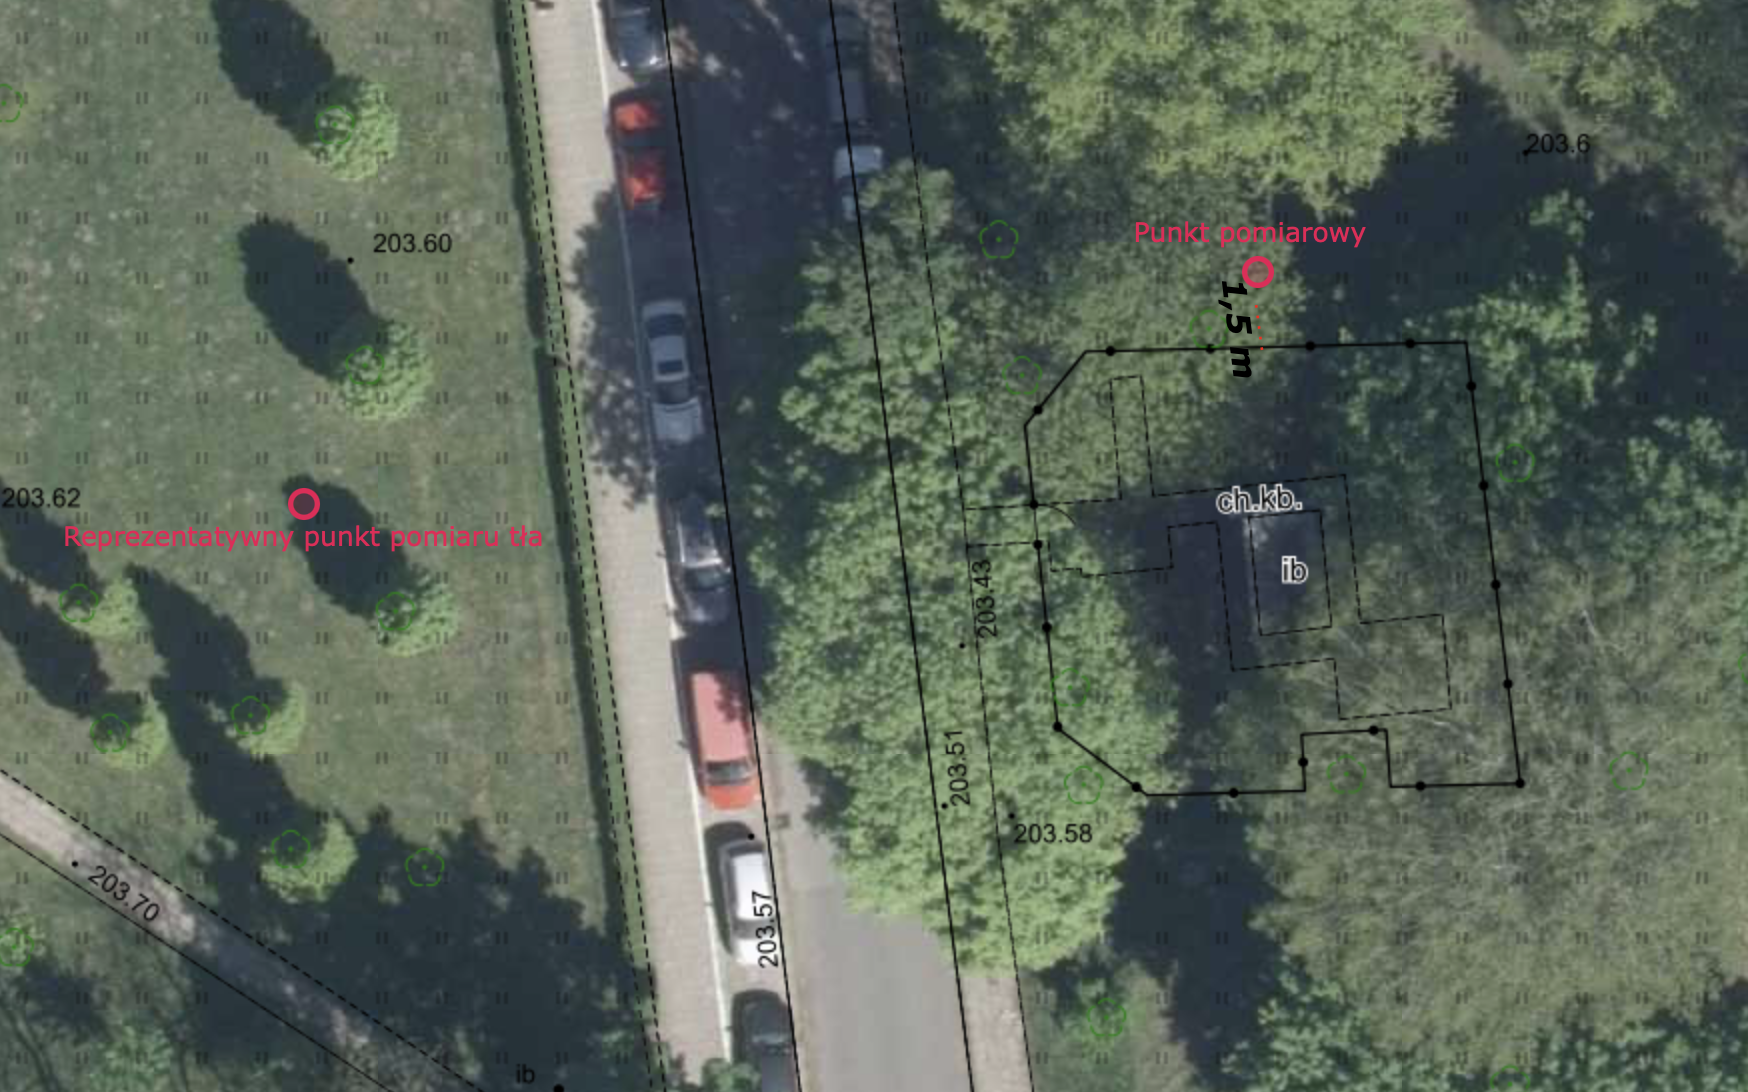
\includegraphics[width=0.8\linewidth]{cwiczenia/01-pomiar-poziomu-cisnienia/figures/punkty_pomiarowe.png}
    \caption{Punkty pomiarowe}
    \label{fig:placeholder}
\end{figure}